\subsection{Mixed Reality und HoloLens}
\label{sec-2-1}

\subsubsection{Mixed Reality}
\label{sec-2-1-1}
\fbox{
	\parbox{\linewidth}{
		\textit{Ziel des Kapitels:}\\
		Begriffsklärung und Einordnung von AR,MR,VR in das Virtual Continuum. Wichtig für die Einordnung von MR in Education in Kap. \ref{sec-2-2}.\\
}}

\begin{figure}[h!]
	\centering
	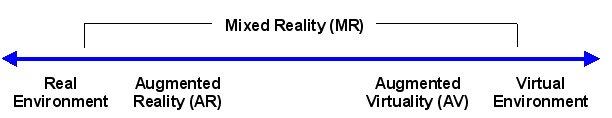
\includegraphics[width=0.9\textwidth]{images/virtual_continuum.png}
	\caption{Virtual Continuum eingeführt von Paul Milgram \cite{Milgram94}}
	\label{img:virtual_continuum}
\end{figure}

\begin{itemize}
	\item Kontinuierliches Spektrum zwischen real und virtuell
	\item MR ist Bereich zwischen völlig real und völlig virtuell, d.h. schließt AR und AV ein
	\item (optional) Einordnung von Beispielen HUD, Snapchat, Fragments, Oculus Rift
	\item Leistungssteigerung im Hardwarebereich und Fortschritte bei AI führt zur Verfügbarkeit von Devices von AR bis VR, daher sehr aktuelles Thema, viel Potential
\end{itemize}


\subsubsection{HoloLens}
\label{sec-2-1-2}
\fbox{
\parbox{\linewidth}{
	\textit{Ziel des Kapitels:}\\
	HoloLens und Mixed Reality Toolkit mit ihrer Technik und Interaktionsweise vorstellen.
}}\\

Die HoloLens ist eine von Microsoft entwickeltes \textit{Head-Mounted Display} (HMD), das seit 2016 auf dem Markt ist. Das Gerät ist in der Lage, virtuelle Darstellungen in der Umgebung des Trägers zu verankern und anzuzeigen. Abbildung \ref{img:hololens} zeigt die Brille in der Standardausführung. Die technischen Eigenschaften und genutzten Techniken des HMDs bringen verschiedene Implikationen und Einschränkungen für Anwendungen auf der HoloLens mit sich. Daher soll im Folgenden auf die technischen Aspekte näher eingegangen werden.\\

\begin{figure}[h!]
	\centering
	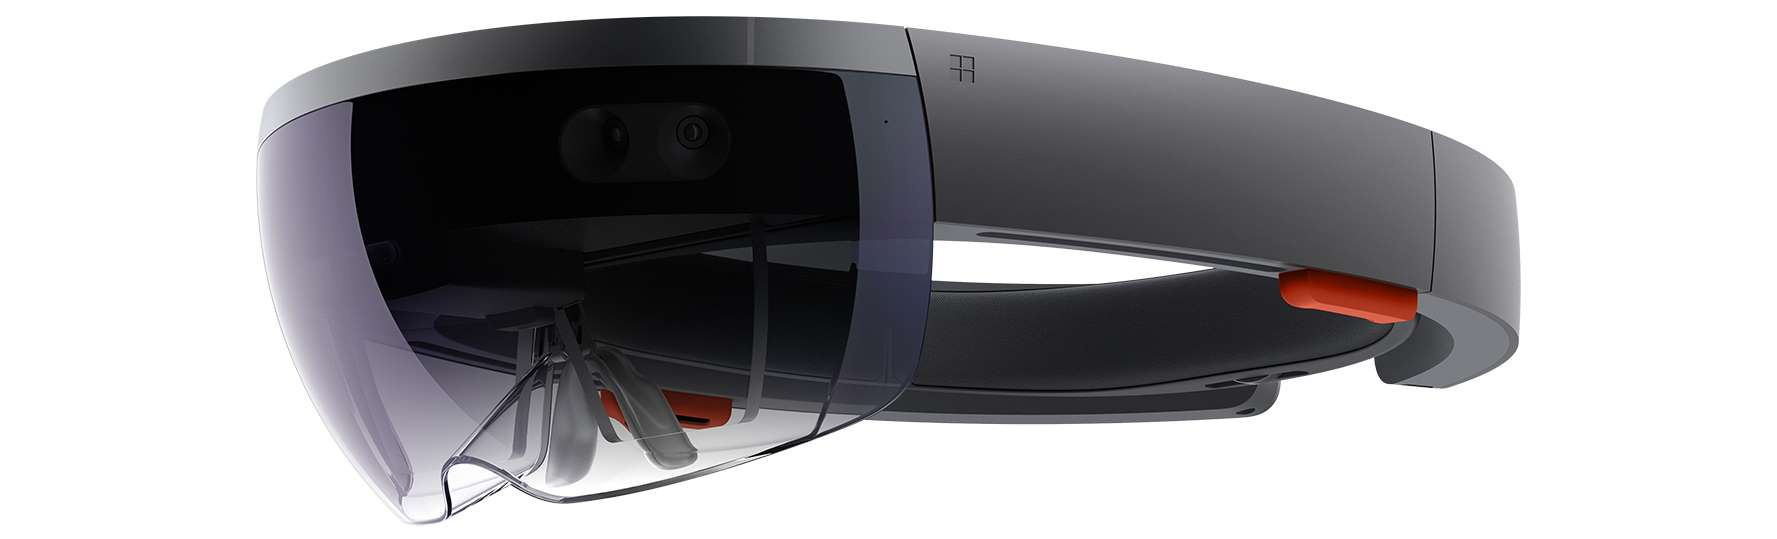
\includegraphics[width=0.9\textwidth]{images/hololens.jpg}
	\caption{Die HoloLens in der Developer Edition (Quelle: Microsoft)}
	%https://www.microsoft.com/de-de/hololens
	\label{img:hololens}
\end{figure}

Bei dem Device handelt es sich um einen eigenständigen Computer, auf dem eine spezielle Version von Windows 10 läuft. Die Brille arbeitet also völlig autonom und ist nicht auf externe Hardware wie z.B. zusätzliche Rechen- und Batterieeinheiten angewiesen.\\

\textbf{Die Hardware}\\
\begin{figure}[h!]
	\centering
	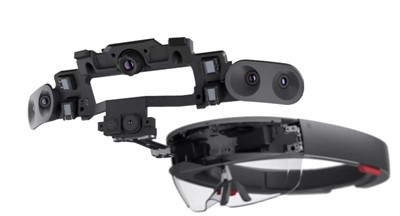
\includegraphics[width=0.9\textwidth]{images/hololens_tech.jpg}
	\caption{Die Sensorik der HoloLens (Quelle: Microsoft)}
	%https://docs.microsoft.com/en-us/windows/mixed-reality/hololens-hardware-details
	\label{img:hololens_tech}
\end{figure}

Einen Überblick über die verwendete Hardware gibt Tabelle \ref{tab:hololens_tech_details}.

\setlength\extrarowheight{2pt}
\begin{table}[htb]
	\centering
	\begin{tabular}{l|l}
		Kategorie & Eigenschaft\\
		\hline
		Anzeige & 720p (HD) in 16:9 Format pro Auge\\
		& 60 Hz Bildwiederholrate\\
		& Blickfeld ca. 32°\\
		Prozessor & Intel 32-Bit Prozessor @ 1.0 GHz\\
		Grafik & Microsoft Holographic Processing Unit (HPU)\\
		Arbeitsspeicher & 2 GB RAM\\
		& 1 GB HPU RAM\\
		Speicher & 64 GB Flash Speicher\\
		Kamera & 2 MP Foto / HD Video Front-Kamera\\
		Sensoren & Inertiale Messeinheit (Accelerometer, Gyroskop, Magnetometer) \\
		& Zwei Stereo Kameras\\
		& 120° x 120° Tiefenkamera\\
		& Vier Mikrofone\\
		& Ambient Light Sensor\\
		Power & 2-3h Akkulaufzeit \\
		Gewicht & 579 Gramm \\
		Konnektivität & WiFi, BLE, USB 2.0, 3.5 mm Audio Jack \\
		Steuerung & Gestensteuerung\\
		& Sprachsteuerung\\
		& HoloLens Klicker, Controller, Maus, Tastatur\\
	\end{tabular}\caption{\label{tab:hololens_tech_details} Spezifikation der HoloLens. Quelle: Microsoft}
\end{table}

\vspace{4px}
\textit{Das Display}\\
Kernstück des Gerätes ist das durchsichtige, stereoskopische Display, mit dem die virtuellen 3D-Objekte angezeigt werden. Durchsichtig bedeutet, dass das Display für Licht von außen durchlässig ist und der Nutzer somit wie durch eine Brille seine Umgebung sehen kann. Virtuelle Objekte werden zusätzlich dazu angezeigt, indem Licht über optische Wellenleiter (Optical Wave Guides) in das Display geleitet wird, welches das Licht dann auf die Augen reflektiert.\\

Anwendungen werden mit 60 Frames pro Sekunde dargestellt. Bei der Anzeige handelt es sich jedoch um ein \textit{Color Sequential Display}, bei dem die drei Farben Rot, Grün und Blau nacheinander dargestellt werden. Pro Bild werden folglich drei Einzelbilder (je eins pro Farbe) gezeigt, was eine Framerate von 240 Hz ergibt.\\

Es handelt sich dabei um ein stereoskopisches Display, bei dem pro Auge separat ein Bild dargestellt wird. So ermöglicht die HoloLens dem Träger das stereoskopische Wahrnehmen dreidimensionaler Objekte. Die beiden Bilder werden in einem festen Abstand von 22 mm zueinander dargestellt. Außerdem beträgt die Distanz, auf die sich die Augen einstellen müssen, damit Bilder als scharf wahrgenommen werden (Akkommodation), etwa zwei Meter und ist ebenfalls fest.\\

\vspace{4px}
\textit{Das Tracking}\\
Um die Hologramme im Raum verankern zu können, benötigt die HoloLens Informationen über ihre exakte Position und Orientierung im Raum. Beides erarbeitet das Gerät allein aus einem Zusammenspiel der verschiedenen internen Sensoren und ist nicht auf externe Markierungen angewiesen, es handelt sich um sogenanntes \textit{Inside-Out Tracking}. Das Vorgehen lässt sich dabei in zwei Bereiche unterteilen: Erfassen der unmittelbaren Umgebung sowie Orientierung anhand der Inertialmesssysteme.\\

Zum einen erstellt die HoloLens ein internes Modell der Oberflächenstruktur der Umgebung. Als Grundlage dazu dienen zum einen eine Tiefenkamera, die anhand der Time-of-Flight von ausgestrahltem Infrarotlicht die Entfernung zu nahegelegenen Oberflächen, die das Licht reflektieren, bestimmt. Zum anderen unterstützen die beiden Stereo-Kameras diese Informationen durch Triangulation von Objekten. Auf diese Weise erarbeitet die Brille ein 3D-Gitternetz, das nach und nach aktualisiert und vervollständigt wird, wenn sich der Träger im Raum bewegt. Anhand dieses sogenannten \textit{Spatial Mapping} wird ein Ankerpunkt für ein im Raum festes Koordinatensystem ausgewählt, dass der Brille als Referenzsystem dient.\\

Um die exakte Position und Ausrichtung der HoloLens nachzuverfolgen kommt außerdem die inertiale Messeinheit zum Einsatz. Die Beschleunigungs-, Rotations- und Magnetflusssensoren ermöglichen Schlussfolgerungen zu Änderungen in Position und Orientierung über eine Zeitdifferenz. Zusammen mit den Informationen aus den optischen Verfahren leitet die Brille so ihre genaue Position und Ausrichtung ab. Darüber hinaus speichert und unterscheidet das Gerät verschiedene Räume anhand der unterschiedlichen Struktur und den dort vorhandenen WLAN Signalen.\\


\textbf{Die Software und Interaktion}\\
\begin{itemize}
	\item Windows 10 Holographic und UWP Apps
	\item Gesten- und Spracherkennung von einigen Handgesten bzw. englischen Wörtern inbegriffen
	\item Raumerkennung und räumliches Verständnis vorhanden
	\item Mixed Reality Toolkit mit wichtigen Funktionen und Beispielen
	\item Entwicklung mit Unity unterstützt
\end{itemize}


\textbf{Implikationen für Anwendungsdesign (kurz)}\\
Genannte technische Details haben Auswirkung auf Nutzung und Design von Anwendungen
\begin{itemize}
	\item Stark spiegelnde oder transparente Materialien ungünstig für das Tracking
	\item Kein Schwarz darstellbar, Helligkeit im Raum relevant, Brille nur in Räumen zu verwenden
	\item Strenge Limitierung von Resourcen für Anwendung, da 60 FPS gehalten werden sollten, also keine komplexen Berechnungen möglich
	\item Abstand, Geschwindigkeit und Größe der Objekte wichtig, Blickwinkel
	\item GGf. Problem mit Sensorik der HoloLens (z.B. Magnetometer)
\end{itemize}
